\documentclass[11pt]{beamer}
\usetheme{Boadilla}
%\usetheme{Berlin}
\usecolortheme{seahorse}
%\usecolortheme{beetle}
\usepackage[utf8]{inputenc}
\usepackage{amsmath}
\usepackage{amsfonts}
\usepackage{amssymb}
\usepackage{natbib}
\usepackage{tcolorbox}
\usepackage{multimedia}
\newcommand{\dif}{\mathrm{d}}
\usepackage{graphicx}
\graphicspath{{Images/}}
\usepackage{media9}
\addmediapath{Animations/}
\newcommand{\folds}{(x_0,y_0)}
\newcommand{\st}{such that }
\newcommand{\wrt}{with respect to }
\newcommand{\vdp}{Van der Pol }
\newcommand{\wlg}{without loss of generality }
\newcommand{\Wlg}{Without loss of generality }


\begin{document}
  

\author{Jonna, Tom, Kieran}
\title{Fast and Slow Dynamics}
%\setbeamercovered{transparent} 
%\setbeamertemplate{navigation symbols}{} 
%\logo{} 
\institute{MIGSAA} 
\date{16/11/2018} 
%\subject{} 
\frame \titlepage
%\begin{frame}
%\begin{itemize}
%\item Dynamical Systems and \vdp
%\item Canards in the \vdp 
%\item Mixed Mode Oscillations (MMO) 
%%\item Canard Points
%\end{itemize}
%		
%\end{frame}


\begin{frame}{ A Quick Reminder: Dynamical Systems}
\begin{onlyenv}<1>
%	\scalebox{1.5}{
\huge
 \[\begin{cases}
 \frac{\dif x}{\dif t}= -y + x^2 - \frac{x^3}{3}\\
 \frac{\dif y}{\dif t}=\epsilon (-\lambda+x)
 \end{cases}\]%}
\end{onlyenv}
\begin{onlyenv}<2>
\begin{columns}
\column{0.6\textwidth}
\begin{figure}
    \centering
\includemedia[width=1\linewidth,height=1\linewidth,activate=pageopen,
passcontext,
transparent,
addresource=vdPbigE.mp4,
flashvars={source=vdPbigE.mp4}
]{}{VPlayer.swf}
\end{figure}
\column{0.4\textwidth}
\[\begin{cases}
 \frac{\dif x}{\dif t}= -y + x^2 - \frac{x^3}{3}\\
 \frac{\dif y}{\dif t}= (-1+x)
 \end{cases}\]
\end{columns}
\end{onlyenv}
\end{frame} 

\begin{frame}{The Van der Pol Equations}
\begin{columns} 
\column{0.5\textwidth}
\begin{figure}
    \centering
\includemedia[width=1\linewidth,height=1\linewidth,activate=pageopen,
passcontext,
transparent,
addresource=vdPe02.mp4,
flashvars={source=vdPe02.mp4}
]{}{VPlayer.swf}
    \caption{Phase Plane of the Van der Pol Equations}
\end{figure}


\column{0.5\textwidth}
\begin{itemize}
    %\item Van der Pol Equations, $\epsilon \rightarrow 0$
    \item Fast System:
    \begin{equation*} 
        % \begin{aligned} 
        \begin{cases}
        \frac{\dif x}{\dif t}&= -y + x^2 - \frac{x^3}{3}\\
        \frac{\dif y}{\dif t}&=\epsilon (-1+x)
        \end{cases}
        % \end{aligned}
        \end{equation*}
\pause
\item Slow System:\\
     \begin{itemize}\item Let $t=\frac{\tau}{\epsilon}$.\end{itemize}
\begin{equation*} 
        \begin{cases}
        \epsilon\frac{\dif x}{\dif \tau} &= -y + x^2 - \frac{x^3}{3}\\ 
        \frac{\dif y}{\dif \tau}&= (-1+x)
        \end{cases}
        \end{equation*}

\end{itemize}
\end{columns}
\end{frame}


\begin{frame}{The Van der Pol Equations, $\epsilon=0$}
\begin{columns} 
\column{0.5\textwidth}
\begin{figure}
    \centering
\includemedia[width=1\linewidth,height=1\linewidth,activate=pageopen,
passcontext,
transparent,
addresource=vdPe001.mp4,
flashvars={source=vdPe001.mp4}
]{}{VPlayer.swf}
    \caption{Phase Plane of the Van der Pol Equations}
\end{figure}
\column{0.5\textwidth}
\begin{itemize}
  
    \item Layer Problem:
    \begin{equation*}
        \begin{cases}
        \frac{\dif x}{\dif t}&= -y + x^2 - \frac{x^3}{3}\\
        \frac{\dif y}{\dif t}&=0
        \end{cases}
        \end{equation*}

\item Reduced System:
\begin{equation*} 
        \begin{cases}
        0 &= -y + x^2 - \frac{x^3}{3}\\ 
        \frac{\dif y}{\dif\tau}&= (-1+x)
        \end{cases}
        \end{equation*}

\end{itemize}
\end{columns}
\end{frame}



\begin{frame}{The Reduced System}
\begin{columns}
\column{0.5\textwidth}
\begin{figure}
    \centering
\includemedia[width=1\linewidth,height=1\linewidth,activate=pageopen,
passcontext,
transparent,
addresource=vdPe001.mp4,
flashvars={source=vdPe001.mp4}
]{}{VPlayer.swf}
    \caption{Phase Plane of the Van der Pol Equations}
\end{figure}
\column{0.5\textwidth}
Reduced System:
\begin{equation*} 
        \begin{cases}
        0 &= -y + x^2 - \frac{x^3}{3} := f(x,y)\\ 
        \frac{\dif y}{\dif \tau}&= (-1+x)
        \end{cases}
        \end{equation*}
\newline
Reduced flow is restricted to:
\begin{align*}
&f=0 \Rightarrow \ \ y = x^2 - \frac{x^3}{3} \ \ \ \ \ \ \
\end{align*}
\newline
\newline
Fold Points:
\begin{itemize}
\item$(x_1^*,y_1^*)= (0,0) $

\item$(x_2^*,y_2^*)=(2,\frac{4}{3})$
\end{itemize}


\end{columns}
\end{frame}





\begin{frame}{The Van der Pol Equations near $(x_1^*,y_1^*)$}
\begin{columns}
\column{0.5\textwidth}
\begin{figure}[h!]
    \centering
    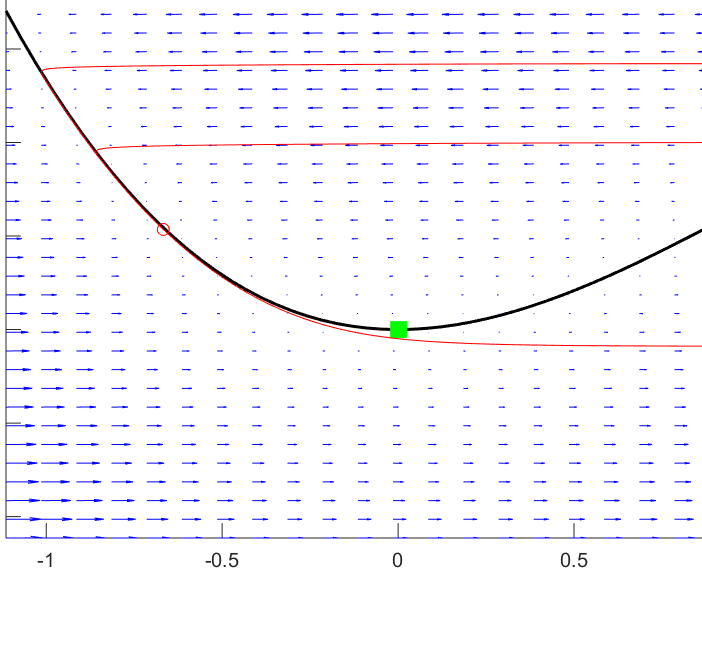
\includegraphics[width=\textwidth]{PPlanecrop.png}
\end{figure}
\column{0.5\textwidth}
Finding $\frac{dx}{d \tau}$ for the reduced system:
\begin{align*}
y&= x^2 - \frac{x^3}{3}\\
\Rightarrow \frac{\dif y}{\dif \tau}  &= \frac{\dif y}{\dif x} \frac{\dif x}{\dif\tau}  = x(2-x)\frac{\dif x}{\dif\tau}\\
\Rightarrow \frac{\dif x}{\dif\tau}&= \frac{\dif y}{\dif\tau}\frac{1}{(2-x)x}
\end{align*}
\newline
%\vspace{0.5cm}
Singularities at $x=0,x=2$.
\end{columns}
\end{frame}



\begin{frame}{The Van der Pol Equations near $(x_1^*,y_1^*)$ }
\begin{columns}
\column{0.5\textwidth}
\begin{figure}[h!]
    \centering
    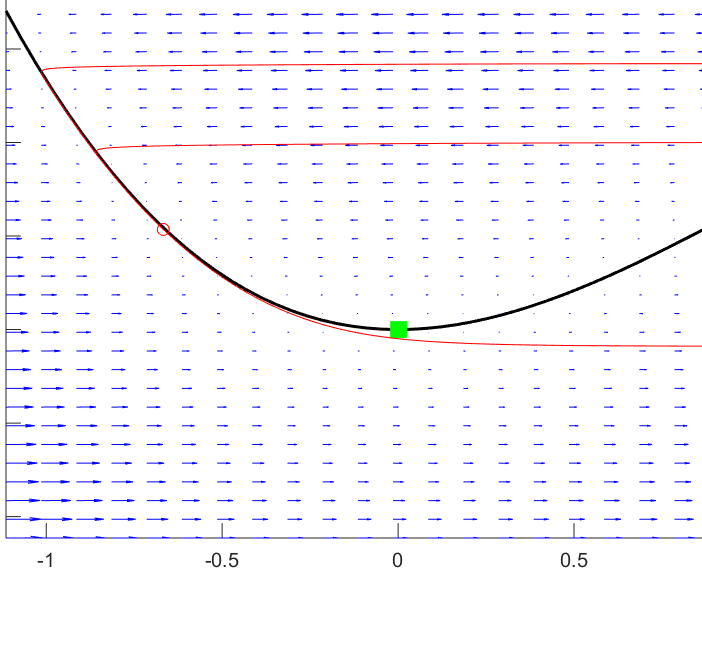
\includegraphics[width=\textwidth]{PPlanecrop.png}
\end{figure}
\column{0.5\textwidth}


Investigating Hyperbolicity:
\begin{align*}
f(x,y)&= -y + x^2 - \frac{x^3}{3}\\
\Rightarrow \frac{\dif f}{\dif x}&= 2x -x^2 \\
&= x(2-x)
\end{align*}
\newline
\newline
Fold Point $(x_1^*,y_1^*)= (0,0) $ is non-hyperbolic.
\end{columns}
\end{frame}




%\begin{onlyenv}<1>
%	\begin{equation*} 
%	\begin{cases}
%	\epsilon\frac{\dif x}{\dif \tau} &= -y + x^2 - \frac{x^3}{3}\\ 
%	\frac{\dif y}{\dif \tau}&= (-1+x)
%	\end{cases}
%	\end{equation*}
%\end{onlyenv}
%
%\begin{onlyenv}<2>
%	\begin{equation*}
%	\begin{cases}
%	\epsilon\frac{\dif x}{\dif \tau} &= -y + x^2 - \frac{x^3}{3}\\ 
%	\frac{\dif y}{\dif \tau}&= (-\lambda+x)
%	\end{cases}
%	\end{equation*}
%\end{onlyenv}
%
%\begin{onlyenv}<3>
	

\begin{frame}{The Blow-up}
\begin{columns}
	\column{0.5\textwidth}
	\begin{figure}
		\centering
		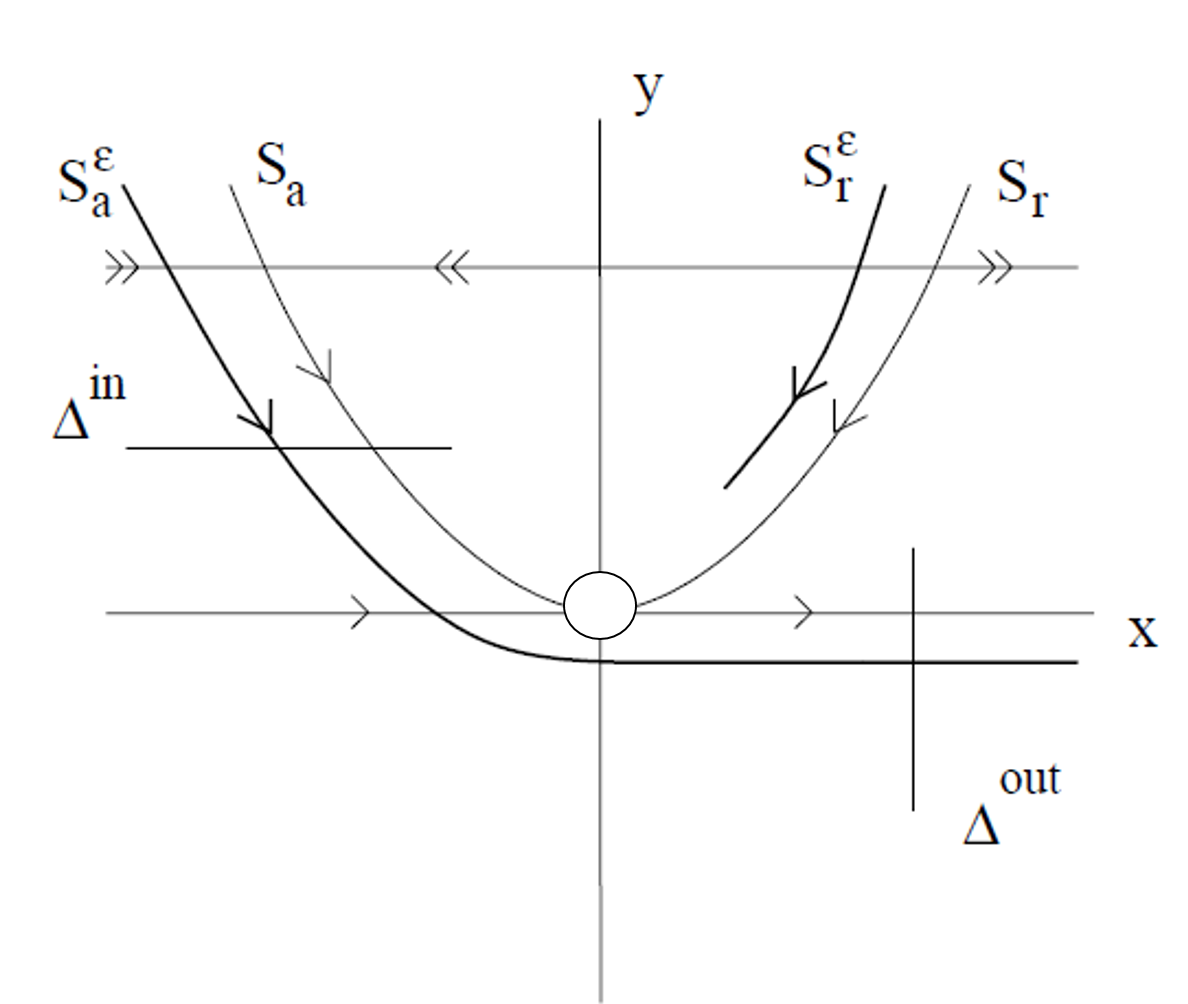
\includegraphics[height=5cm, width=5cm]{Blow_up.png}
		\caption{Blow up of our fold point (Kuehn, Multiple Time Scale Dynamics)}
	\end{figure}\column{0.5\textwidth}
	\begin{itemize}
		
		\item The radius $r=0$
		\item Coordinate transformation
		\begin{itemize}
			\item $x=r_ix_i, \ y=r_i^2y_i, \ \epsilon=r_i^3\epsilon_i$\\
		\end{itemize}
		%\item Letting $r$ go to zero to describe flow on surface of blown up point $(x_1*,y_1*)$.
		\item Analysing our blow up
	\end{itemize}
\end{columns}
\end{frame}

\begin{frame}{Charts Motivation}
\begin{columns}
\column{0.5\textwidth}
\begin{figure}
	\centering
	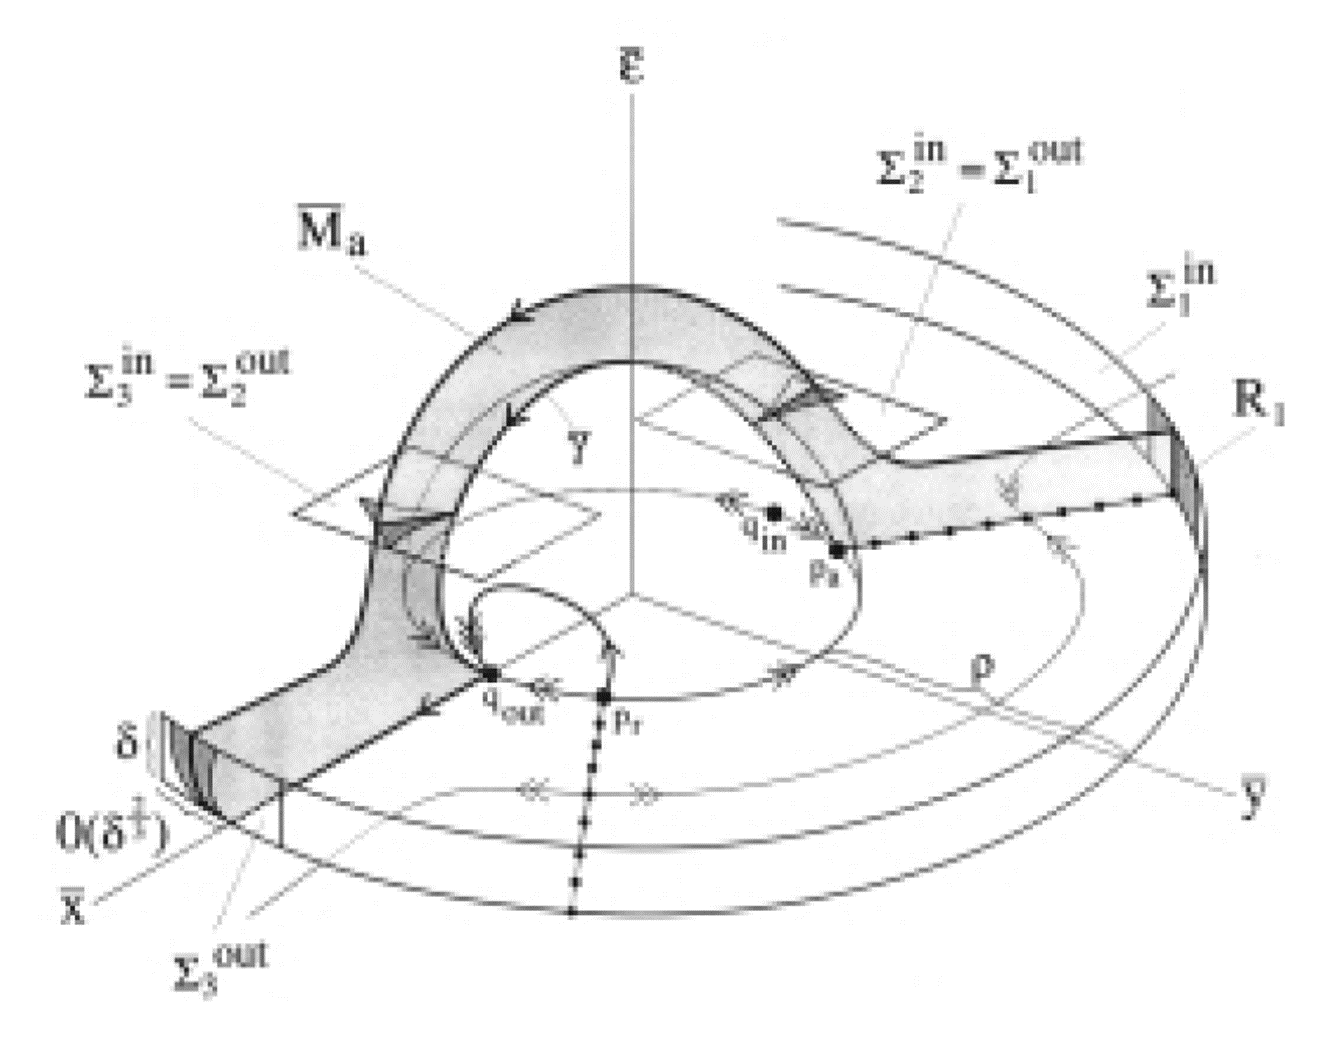
\includegraphics[height=5cm,width=6cm]{Charts.png}
	\caption{Sketch of the coordinate charts (Kuehn, Multiple Time Scale Dynamics)}
\end{figure}    \column{0.5\textwidth}
\begin{itemize}
	\item What are charts?
	\item Why use charts?
	\begin{itemize}
		\item Simplifies our singularity
		\item Magnifies our flow 
	\end{itemize}
	\item Transition Maps $\Pi_1\to \Pi_2\to \Pi_3$
\end{itemize}

\end{columns}
\end{frame}

\begin{frame}{Dynamics on $K_2$}
\begin{columns}
\column{0.5\textwidth}
\begin{figure}
\centering
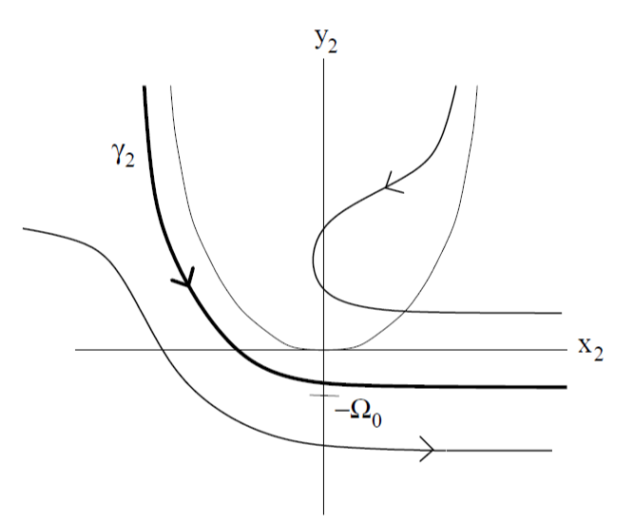
\includegraphics[height=4cm,width=6cm]{Dynamics_in_K2.png}
\caption{Phase portrait for $\bar{\epsilon}=0$ (Kuehn, Multiple Time Scale Dynamics)}

\end{figure}\column{0.5\textwidth}
\begin{itemize}
\item Transformed Van der Pol equations on $ \epsilon=1$:
\begin{equation*}
\begin{cases}
x_2' &= x_2^2-y_2+O(r_2)\\
y_2' &= -1+O(r_2)\\
r'_2&=0
\end{cases}
\end{equation*}
%\item $ x_2' = x_2^2-y_2$
%\item $y_2' = -1$
%\item $r'_2=0$
\item Riccati Equations.
\begin{itemize}
	\item Asymptotic solution.
\end{itemize}
\item Transition map, $\Pi_2$, exists
%\begin{itemize}
%\item Mapping trajectories coming from K1 onto trajectories going to K3.
%\item Trajectories follow a Riccati solution on K2.

%\end{itemize}
\end{itemize}
\end{columns}
\end{frame}

\begin{frame}{Dynamics on $K_1$ and $K_3$}
\begin{columns}
\column{0.5\textwidth}
\begin{figure}
\centering
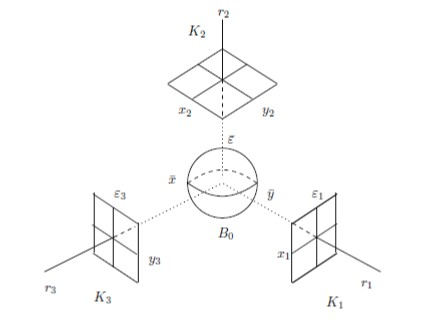
\includegraphics[height=4cm,width=6cm]{charts-ball}
\caption{The attracting branch connecting to the blow up.}
\end{figure}\column{0.5\textwidth}
\begin{itemize}
\item Dynamics on $K_1$:
% \begin{equation*}
%     \begin{aligned}
%         &  x_2' = x_2^2-y_2+O(r_2)\\
%          &y_2' = -1+O(r_2)\\
%         &r'_2=0
%     \end{aligned}
% \end{equation*}
%\item $ x_2' = x_2^2-y_2$
%\item $y_2' = -1$
%\item $r'_2=0$
\begin{itemize}
\item Centre Manifold Theorem

% \item Finding equilibria, eigenvalues and eigenvectors
\end{itemize}
% \item Existence of $\Pi$ connecting $S^a \ \text{and} \ K_2$.
\item Dynamics in $K_3$
\begin{itemize}
%\item Mapping trajectories coming from K1 onto trajectories going to K3.
%\item Trajectories follow a Riccati solution on K2.
\item Resonance
\end{itemize}
\end{itemize}
\end{columns}
\end{frame}



\begin{frame}{Global Solution}
\begin{columns}
\column{0.5\textwidth}
\begin{figure}

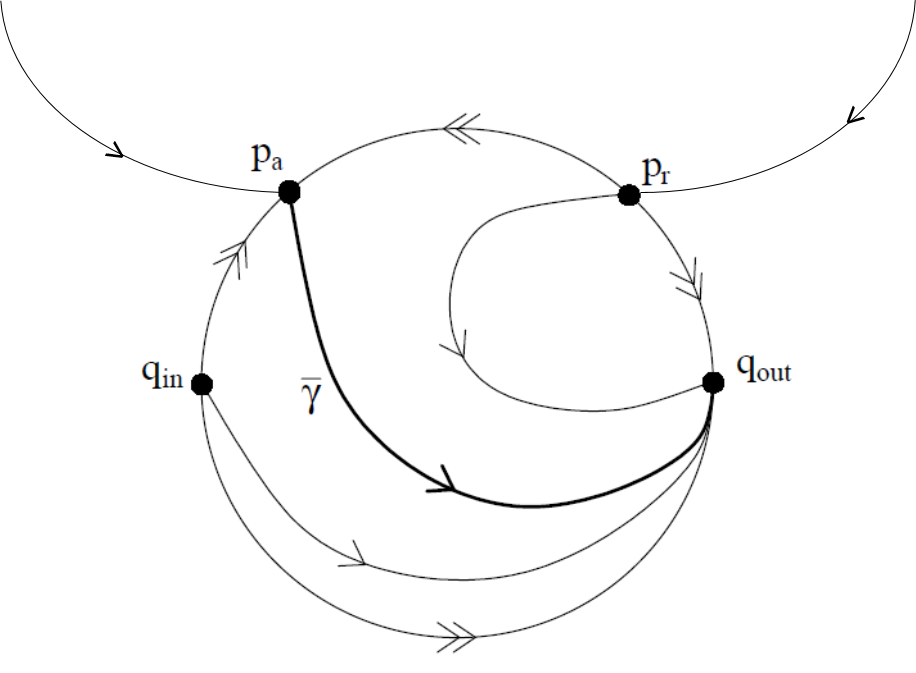
\includegraphics[height=5cm,width=7cm]{Blow_up_fold.png}
\caption{Global dynamics of the blown up system (Kuehn, Multiple Time Scale Dynamics)}

\end{figure}\column{0.5\textwidth}
\begin{itemize}
%\item The maps $\Pi_1, \Pi_2, \Pi_3$ can be combined into a global map $\Pi$ using the variable transformations.
\item $\Pi$ describes the global transition of trajectories.
\begin{itemize}
\item $\Pi=\Pi_3\circ\kappa_{23}\circ\Pi_2\circ\kappa_{12}\circ\Pi_1$
\end{itemize}
% \item Riccati flow at $\bar{\gamma}.$
\item What does $q_{out}$ do?
% \item This describes the flow at $(x^*,y^*)=(0,0)$. %(not on but around???)
\end{itemize}
\end{columns}
\end{frame}%
%\begin{frame}{Dynamics on $K_2$}
%\begin{columns}
%\column{0.35\textwidth}
%\begin{figure}
%    \centering
%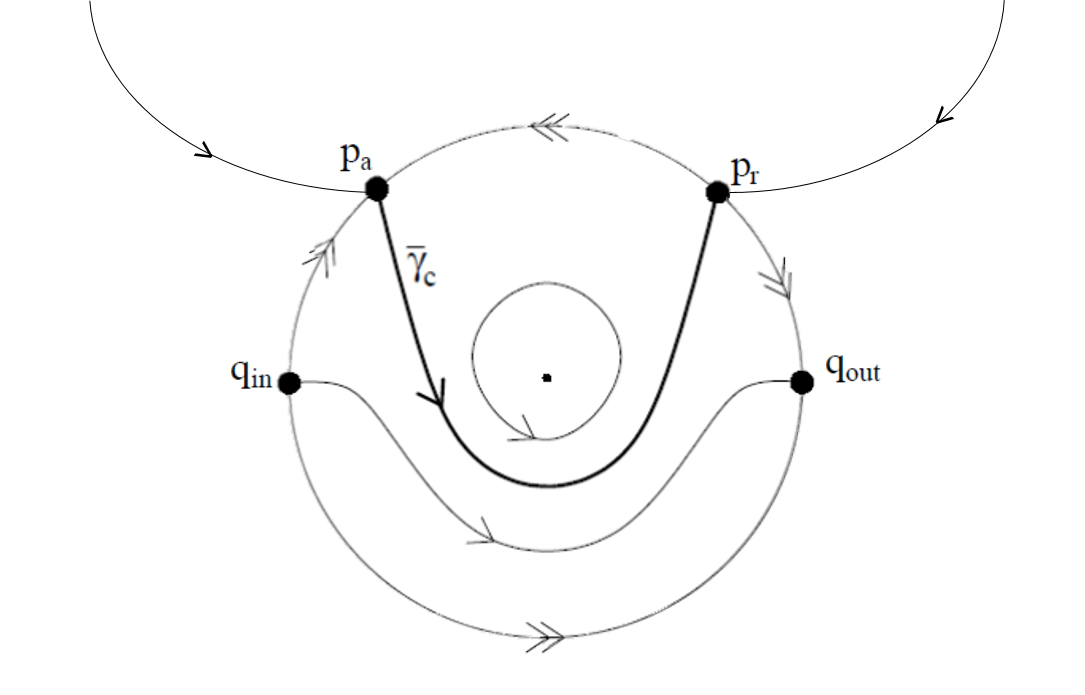
\includegraphics[height=4cm,width=5cm]{Images/pres-cancard}
%	\caption{Trajectories in the blow up (Kuehn, Multiple Time Scale Dynamics)}
%\end{figure}\column{0.65\textwidth}
%\begin{itemize}
%\item Transformed Van der Pol equations on $ \epsilon=1$:
%\begin{equation*}
%    \begin{cases}
%        x'_2&=-y_2+x_2^2\\
%         y_2'&=x_2-\lambda_2\\
%        r'_2&=0\\
%        \lambda'_2&=0\\
%    \end{cases}
%%     G(x_2,y_2)=(G_1(x_1,y_1),G_2(x_2,y_2))^T=(-\frac{x^2_2}{3},0)^T
%\end{equation*}
%%\item $ x_2' = x_2^2-y_2$
%%\item $y_2' = -1$
%%\item $r'_2=0$
%%\item Matrix of high order terms.
%%\begin{itemize}
%%\item  $G(x_2,y_2)=(-\frac{x^2_2}{3},0)^T$
%%\end{itemize}
%\item Constant of Motion in $ K_2 $
%\begin{itemize}
%	\item $H(x_2,y_2)=\frac{1}{2}e^{(-2y_2)}\left(y_2-x^2_2+\frac{1}{2}\right)$
%\end{itemize}
%%\begin{itemize}
%%\item Mapping trajectories coming from K1 onto trajectories going to K3.
%%\item Trajectories follow a Riccati solution on K2.
%
%%\end{itemize}
%\end{itemize}
%\end{columns}
%\end{frame}
%
%\begin{frame}{Global Solution}
%\begin{columns}
%	\column{0.5\textwidth}
%	\begin{figure}
%		\centering
%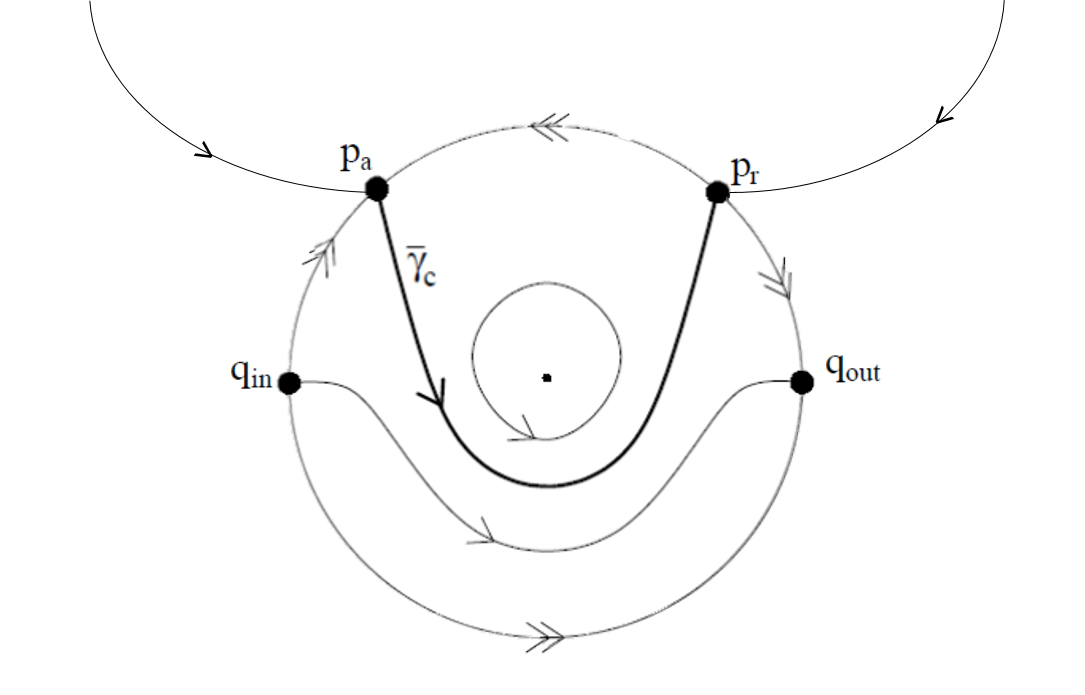
\includegraphics[height=4cm,width=6cm]{Images/pres-cancard}
%		\caption{Trajectories in the blow up (Kuehn, Multiple Time Scale Dynamics)}
%		
%	\end{figure}\column{0.5\textwidth}
%	\begin{itemize}
%%		\item Transformed Van der Pol equations on $ \epsilon=1$:
%%		\begin{equation*}
%%		\begin{cases}
%%			r_1'&=\frac{\epsilon}{2}(r_1x_1-r_1\lambda_1), \\
%%		% \label{canard: r1}
%%		x_1'&=-1+x_1^2-\frac{x_1\epsilon_1F}{2},\\
%%		\epsilon'&=-\epsilon_1^2F,\\
%%		\lambda'_1&=-\frac{\lambda_1\epsilon_1F}{2}.
%%		\end{cases}
%%		%     G(x_2,y_2)=(G_1(x_1,y_1),G_2(x_2,y_2))^T=(-\frac{x^2_2}{3},0)^T
%%		\end{equation*}
%%		%\item $ x_2' = x_2^2-y_2$
%%		%\item $y_2' = -1$
%%		%\item $r'_2=0$
%%		%\item Matrix of high order terms.
%%		%\begin{itemize}
%%		%\item  $G(x_2,y_2)=(-\frac{x^2_2}{3},0)^T$
%%		%\end{itemize}
%		\item Trajectories
%		\begin{itemize}
%			\item Hopf Bifurcation
%			\item Jumps
%		\end{itemize}
%		%\begin{itemize}
%		%\item Mapping trajectories coming from K1 onto trajectories going to K3.
%		%\item Trajectories follow a Riccati solution on K2.
%		
%		%\end{itemize}
%	\end{itemize}
%\end{columns}
%\end{frame}
%
%
%
%\begin{frame}{Effects of a Canard}
%\begin{columns}
%\column{0.5\textwidth}
%\begin{figure}
%    
%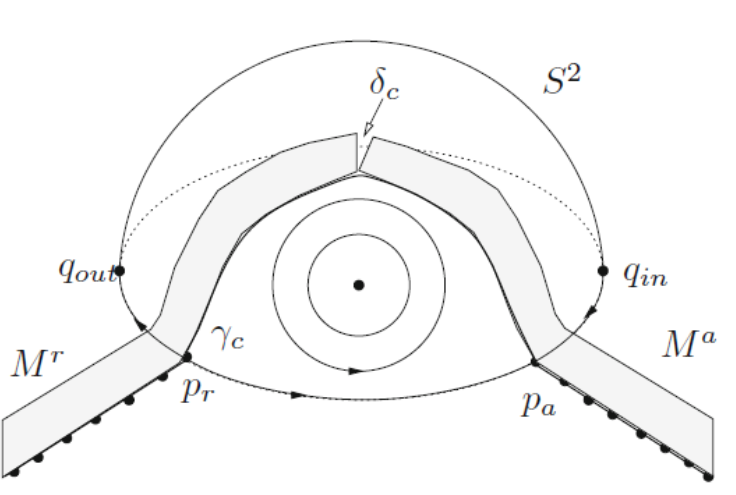
\includegraphics[height=5cm,width=7cm]{Images/Separation}
%    \caption{Separation of $ M_a $ and $ M_r $ (Kuehn, Multiple Time Scale Dynamics).}
%
%\end{figure}\column{0.4\textwidth}
%\begin{itemize}
%%\item The maps $\Pi_1, \Pi_2, \Pi_3$ can be combined into a global map $\Pi$ using the variable transformations.
%\item Hopf Bifurcation
%\item Splitting 
%
%%\begin{itemize}
%%    \item $\Pi=\Pi_3\circ\kappa_{23}\circ\Pi_2\circ\kappa_{12}\circ\Pi_1$
%%\end{itemize}
%%% \item Riccati flow at $\bar{\gamma}.$
%%\item What does $q_{out}$ do?
%%% \item This describes the flow at $(x^*,y^*)=(0,0)$. %(not on but around???)
%\end{itemize}
%\end{columns}
%\end{frame}
%\\
\begin{frame}{Canard Points in the \vdp}
\begin{columns}
	\column{0.5\textwidth}
	\begin{figure}
		\centering
		\includemedia[width=1\linewidth,height=1\linewidth,activate=pageopen,
		passcontext,
		transparent,
		addresource=vdPhopf.mp4,
		flashvars={source=vdPhopf.mp4}
		]{}{VPlayer.swf}
		
	\end{figure}
	\column{0.5\textwidth}
	\begin{figure}
		\centering
		\includemedia[width=1\linewidth,height=1\linewidth,activate=pageopen,
		passcontext,
		transparent,
		addresource=vdPe001.mp4,
		flashvars={source=vdPe001.mp4}
		]{}{VPlayer.swf}
		%\caption{Phase Plane of the Van der Pol Equations}
	\end{figure}
	
\end{columns}
\begin{equation*} 
\begin{cases}
\epsilon\frac{\dif x}{\dif \tau} &= -y + x^2 - \frac{x^3}{3}\\ 
\frac{\dif y}{\dif \tau}&= (-\lambda+x)
\end{cases}
\end{equation*}
\end{frame}

\begin{frame}{Mixed Mode Oscillations (MMO's)}
\begin{columns}
	\column{0.6\linewidth}
	\begin{figure}
		
		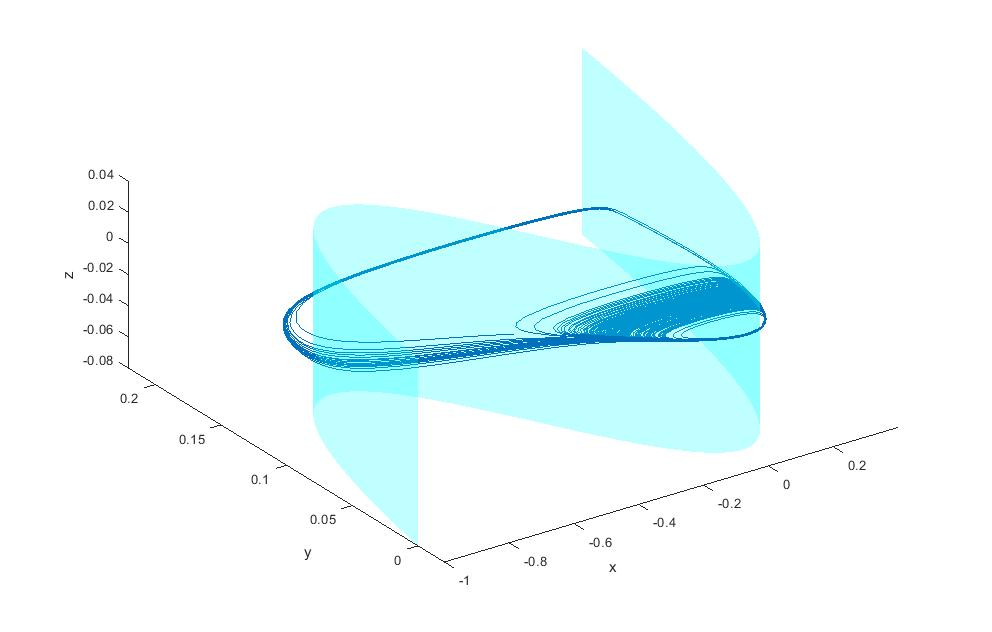
\includegraphics[width=\textwidth]{Images/chaoticEvdp}
		
		
	\end{figure}\column{0.4\linewidth}
\begin{figure}
	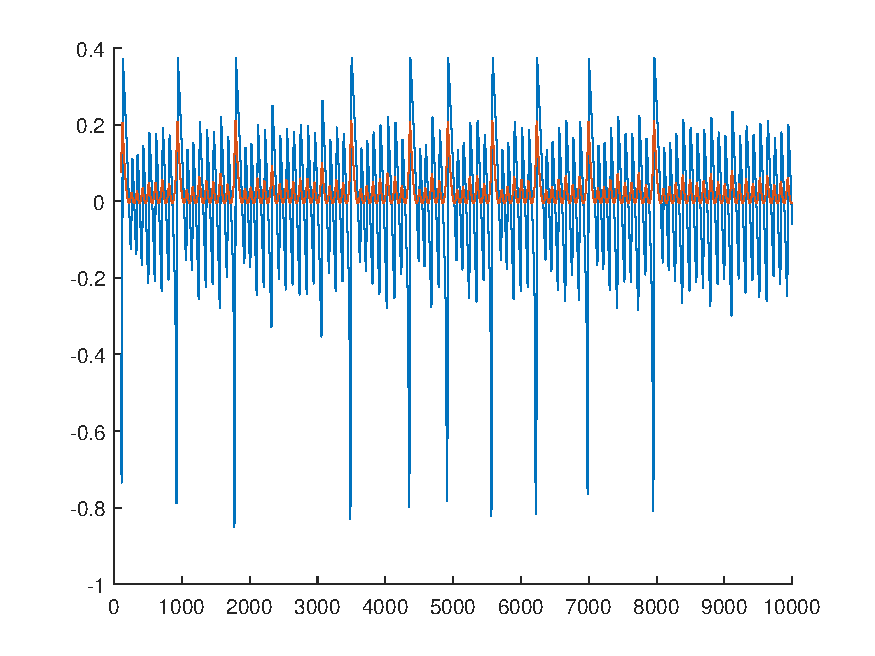
\includegraphics[width=\textwidth]{Images/eVDPts}
	
\end{figure}

\end{columns}
\begin{center} Phase Portrait and Time Series of chaotic MMO \end{center}
\end{frame}


\begin{frame}{Mixed Mode Oscillations (MMO's)}
%\begin{frame}{Effects of a Canard}
\begin{columns}
	\column{0.5\textwidth}
	\begin{figure}
		
		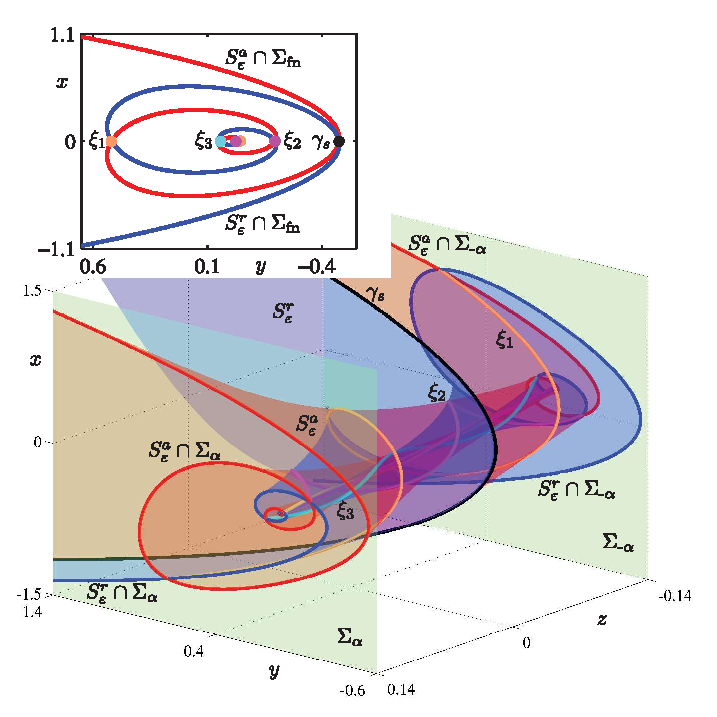
\includegraphics[height=5cm,width=6cm]{Images/MMO-spirals}
		\caption{Canards in the normal form system (Desroches et al., 2015)}
		
	\end{figure}\column{0.4\textwidth}
	\begin{itemize}
		\item Normal Form:
		\begin{equation*}
			 \begin{cases}
			\dot{x}&=y-x^2\\
			\dot{y}&=z-x\\
			\dot{z}&=-\nu
			\end{cases} 
		\end{equation*}
		\item MMO due to a Folded Node 
	\end{itemize}
\end{columns}
\end{frame}

\begin{frame}{Conclusion}
\begin{onlyenv}<1>
\end{onlyenv}
\begin{onlyenv}<2>
\begin{columns}
\column{0.5\linewidth}
	\begin{figure}
		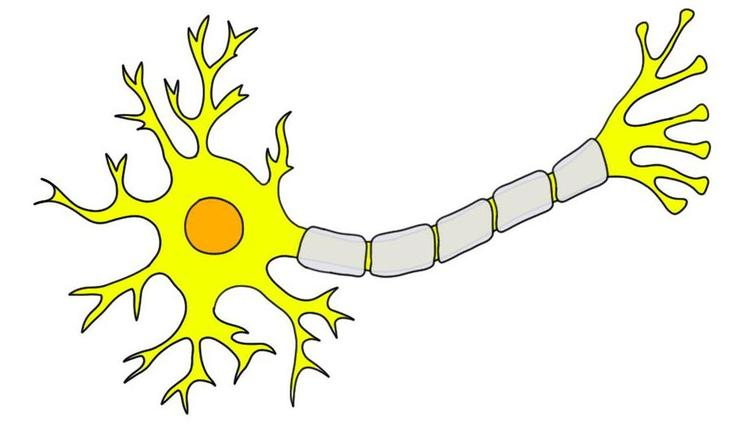
\includegraphics[width=\linewidth]{Images/neuron}
	\end{figure}%
\column{0.5\linewidth}
		\begin{figure}
		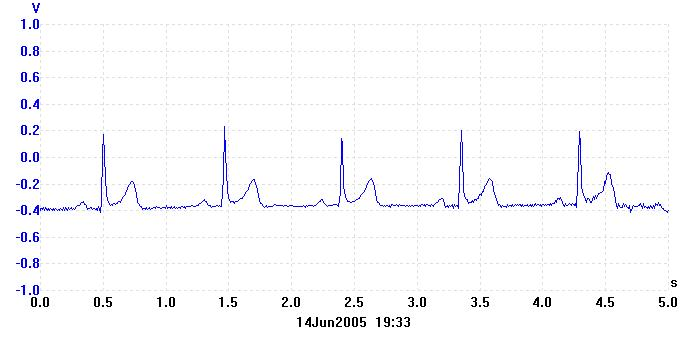
\includegraphics[width=\linewidth]{Images/ECG}
	\end{figure}%
\end{columns}
\end{onlyenv}


\end{frame}


\end{document}